% Options for packages loaded elsewhere
\PassOptionsToPackage{unicode}{hyperref}
\PassOptionsToPackage{hyphens}{url}
\documentclass[
]{article}
\usepackage{xcolor}
\usepackage[margin=2.5cm]{geometry}
\usepackage{amsmath,amssymb}
\setcounter{secnumdepth}{-\maxdimen} % remove section numbering
\usepackage{iftex}
\ifPDFTeX
  \usepackage[T1]{fontenc}
  \usepackage[utf8]{inputenc}
  \usepackage{textcomp} % provide euro and other symbols
\else % if luatex or xetex
  \usepackage{unicode-math} % this also loads fontspec
  \defaultfontfeatures{Scale=MatchLowercase}
  \defaultfontfeatures[\rmfamily]{Ligatures=TeX,Scale=1}
\fi
\usepackage{lmodern}
\ifPDFTeX\else
  % xetex/luatex font selection
\fi
% Use upquote if available, for straight quotes in verbatim environments
\IfFileExists{upquote.sty}{\usepackage{upquote}}{}
\IfFileExists{microtype.sty}{% use microtype if available
  \usepackage[]{microtype}
  \UseMicrotypeSet[protrusion]{basicmath} % disable protrusion for tt fonts
}{}
\makeatletter
\@ifundefined{KOMAClassName}{% if non-KOMA class
  \IfFileExists{parskip.sty}{%
    \usepackage{parskip}
  }{% else
    \setlength{\parindent}{0pt}
    \setlength{\parskip}{6pt plus 2pt minus 1pt}}
}{% if KOMA class
  \KOMAoptions{parskip=half}}
\makeatother
\usepackage{graphicx}
\makeatletter
\newsavebox\pandoc@box
\newcommand*\pandocbounded[1]{% scales image to fit in text height/width
  \sbox\pandoc@box{#1}%
  \Gscale@div\@tempa{\textheight}{\dimexpr\ht\pandoc@box+\dp\pandoc@box\relax}%
  \Gscale@div\@tempb{\linewidth}{\wd\pandoc@box}%
  \ifdim\@tempb\p@<\@tempa\p@\let\@tempa\@tempb\fi% select the smaller of both
  \ifdim\@tempa\p@<\p@\scalebox{\@tempa}{\usebox\pandoc@box}%
  \else\usebox{\pandoc@box}%
  \fi%
}
% Set default figure placement to htbp
\def\fps@figure{htbp}
\makeatother
\setlength{\emergencystretch}{3em} % prevent overfull lines
\providecommand{\tightlist}{%
  \setlength{\itemsep}{0pt}\setlength{\parskip}{0pt}}
\usepackage{bookmark}
\IfFileExists{xurl.sty}{\usepackage{xurl}}{} % add URL line breaks if available
\urlstyle{same}
\hypersetup{
  hidelinks,
  pdfcreator={LaTeX via pandoc}}

\author{}
\date{}

\begin{document}

\section{A Thought Experiment on Double-Slit Interference from a Source
with Positional Fluctuation --- Push-forward of the Source-Position
Distribution to the Fringe-Shift Distribution (Shape
Preservation)}\label{a-thought-experiment-on-double-slit-interference-from-a-source-with-positional-fluctuation-push-forward-of-the-source-position-distribution-to-the-fringe-shift-distribution-shape-preservation}

\textbf{Noriaki Kihara}

\emph{This paper is a \textbf{thought experiment (model calculation)},
not a measurement. It contains no claim that overturns established
physics (standard wave optics / quantum mechanics). For a specified
geometry, it illustrates by exact analysis and numerical computation how
the probability distribution of the source position is mapped onto the
probability distribution of the far-field interference-fringe shift over
repeated trials.}

Version v0.3 (2026-06-29) DOI (Version): 10.5281/zenodo.21035809 DOI
(Concept): 10.5281/zenodo.21035808 Zenodo:
https://zenodo.org/records/21035809

\begin{center}\rule{0.5\linewidth}{0.5pt}\end{center}

\subsection{Abstract}\label{abstract}

We assume a stationary point source whose position has a fluctuation of
order \(\pm\lambda/2\) (half a wavelength), and consider far-field
interference through a double slit. In a single trial with a given
source position \(y\), the interference fringe appears as a single
fringe of \textbf{identical shape, merely shifted left or right by the
pure geometric path difference} (the wavelength is \(\lambda_0\)
everywhere; no frequency shift is involved). The central-peak shift
\(u(y)\) is a \textbf{nearly linear map} of the source position.

The claim of this paper is the following. \textbf{In repeated
observation where the source position \(y\) is drawn randomly each trial
from a probability distribution \(P(y)\), the probability distribution
of the per-trial fringe shift \(u\) is the push-forward
\(\rho(u)=P(y(u))\,|dy/du|\) of \(P\); because the map \(u(y)\) is
linear, the shape of \(P\) is preserved whatever it is.} This is not the
derivation of a new probability law but an illustration of a change of
variables (push-forward) by which the input distribution is mapped,
through a nearly linear geometric map, onto the distribution of the
shift. We use \(P(y)=\cos^2(\pi y/\lambda)\) as a concrete example and
show that the shift distribution is the same-shape \(\cos^2\). The
\(\sim2\text{–}3\%\) departure from this shape arises from the
non-paraxial nonlinearity of the map \(u(y)\) (the non-paraxial scale
\(\tfrac12\tan^2\theta\approx3\%\)) and vanishes in the paraxial limit
\(W/L\to0\).

As an important caveat, this distribution is \textbf{not a property of a
single observed image}. A single trial yields just one shift value (one
fringe). Moreover, the image obtained by \textbf{accumulating} the
intensity of many trials on one screen is a \textbf{single fringe of
reduced visibility} convolved with the shift, not the shape of the input
distribution. The shape appears when one reads the shift each trial and
builds a histogram over repetitions (assuming the source position is
quasi-static within a trial and fluctuates between trials).

\begin{center}\rule{0.5\linewidth}{0.5pt}\end{center}

\subsection{1. Introduction}\label{introduction}

Double-slit interference is a basic stage for thought experiments in
both wave optics and quantum mechanics. Here we ask what statistics
appear in the fringe shift over repeated observation when the source
position fluctuates.

To anticipate the conclusion: each trial merely shifts the same fringe,
and the shift is a nearly linear map of the source position. Therefore,
if the source position is repeatedly drawn from a distribution \(P(y)\),
\textbf{the shift distribution is the push-forward of \(P\) and
preserves the same shape in the paraxial regime}. This is not the
derivation of a new probability law but an illustration of the change of
variables that maps the input distribution onto the observed statistic
(the shift). Taking \(P(y)=\cos^2(\pi y/\lambda)\) as an example, we
show that the shift distribution is the same-shape \(\cos^2\) and that
the departure is limited to the non-paraxial
\(\tfrac12\tan^2\theta\approx3\%\). This is a thought experiment;
everything is an exact computation on the specified geometry.

\begin{center}\rule{0.5\linewidth}{0.5pt}\end{center}

\subsection{2. Experimental conditions}\label{experimental-conditions}

\subsubsection{2.1 Overall configuration}\label{overall-configuration}

A single point source \(S\) (wavelength \(\lambda_0=1\), speed of light
\(c=1\)) illuminates a double slit at distance \(L=10\). The slit
separation is \(W=5\), and the slits are placed symmetrically about the
optical axis (\(y=\pm W/2=\pm2.5\)). Each slit subtends a half-angle
\(\theta=\arctan(0.25)\approx14.04^\circ\) from the source about the
axis. The screen is far (\(D\gg L\), Fraunhofer regime).

\begin{figure}
\centering
\pandocbounded{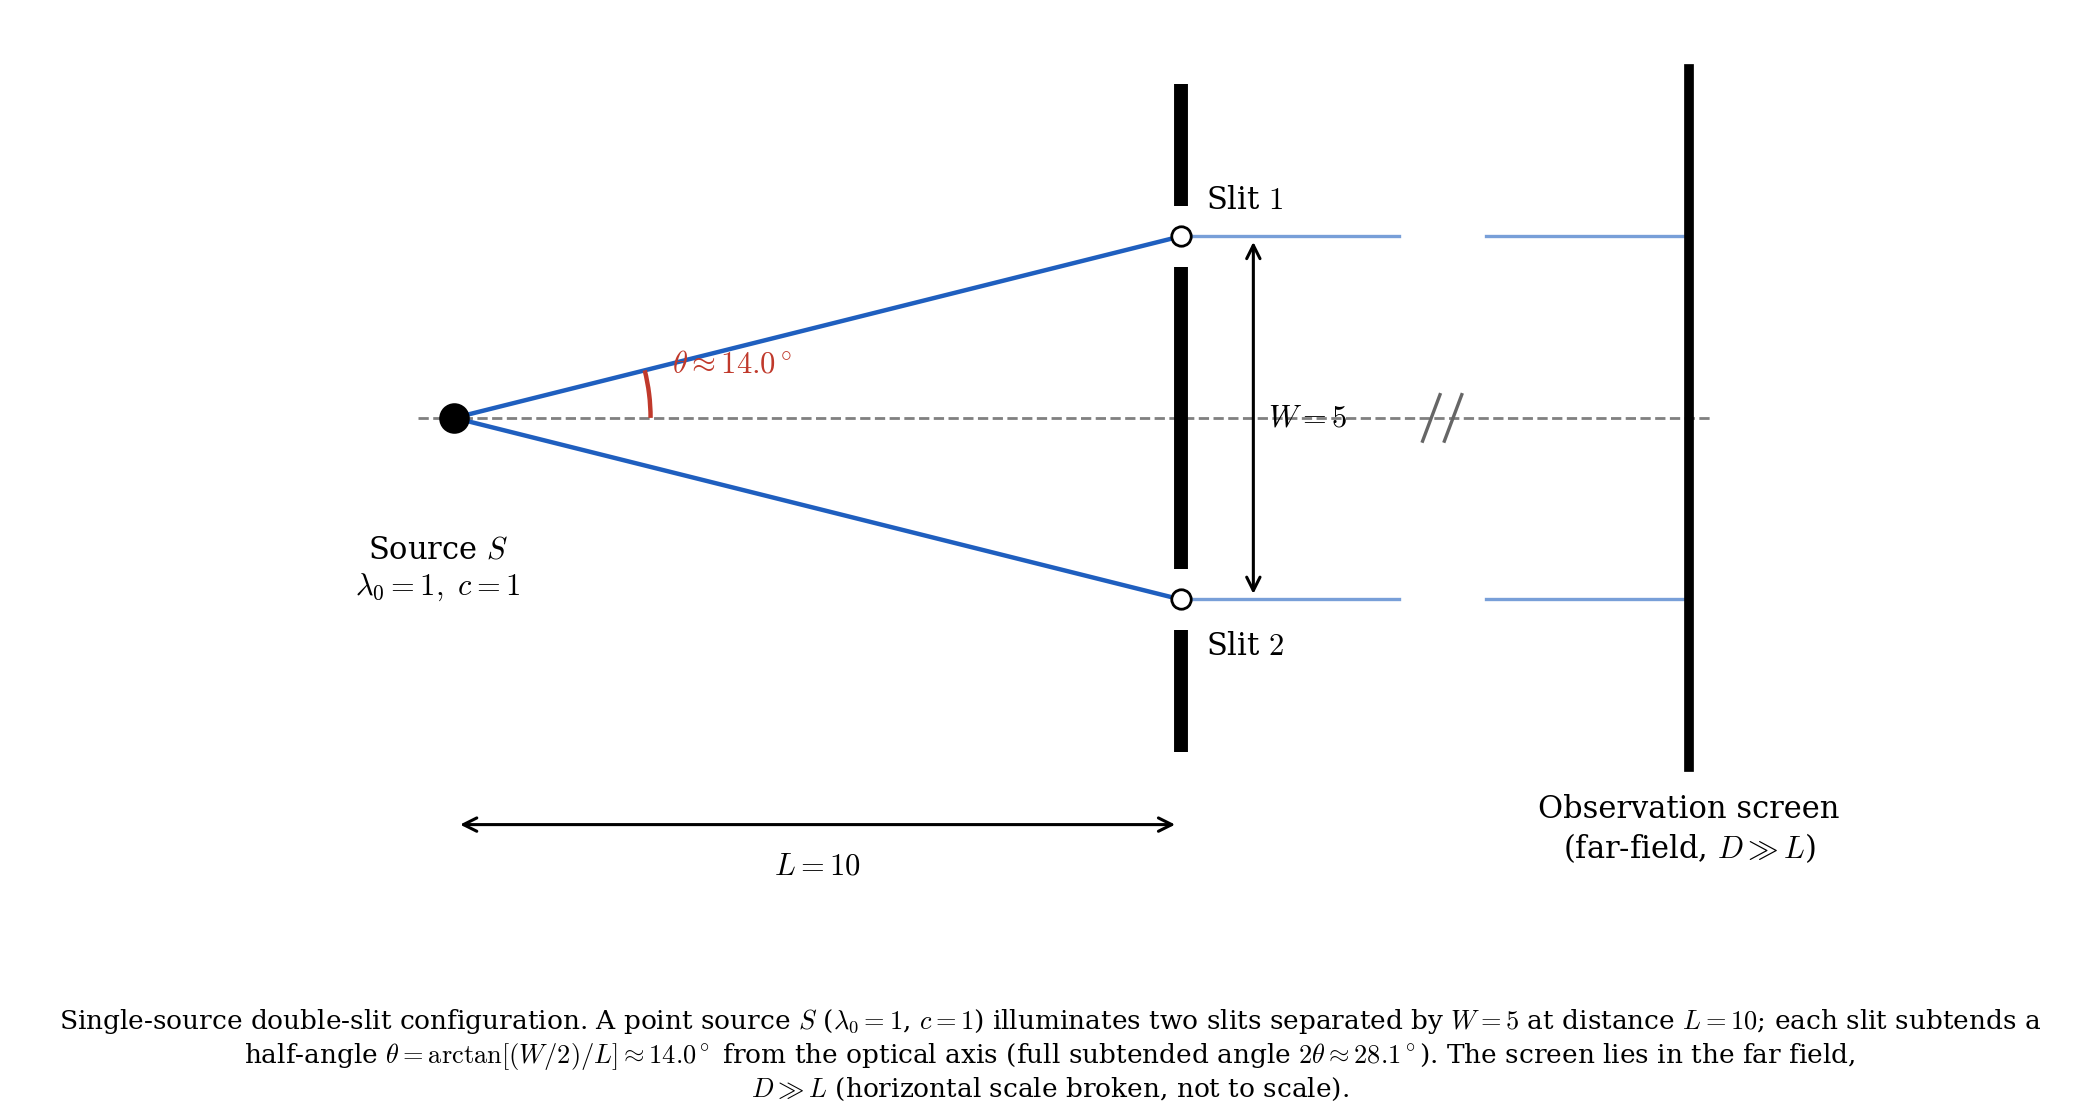
\includegraphics[keepaspectratio,alt={Fig 1 overall configuration}]{fig_setup_double_slit.png}}
\caption{Fig 1 overall configuration}
\end{figure}

\emph{Fig 1: Overall configuration of single source and double slit
(\(L=10\), \(W=5\), \(\lambda_0=1\), \(c=1\)). Each slit subtends
half-angle \(\theta\approx14^\circ\) from the axis. The screen is far
(the transverse direction is broken / not to scale).}

\subsubsection{2.2 Positional fluctuation of the
source}\label{positional-fluctuation-of-the-source}

We assign the source position an uncertainty of radius \(\lambda/2\) and
take, as a concrete example, the probability distribution of the
transverse position \(y\) (parallel to the screen) to be

\[P(y)=\cos^2\!\Big(\frac{\pi y}{\lambda}\Big),\qquad y\in[-\tfrac{\lambda}{2},\,\tfrac{\lambda}{2}]\]

(a centrally-peaked bell that is zero at \(\pm\lambda/2\)). We take the
positional scale \(\lambda\) equal to the optical wavelength
\(\lambda_0\) (\(\lambda=\lambda_0=1\)). We treat this distribution as
input and do not ask its origin. The source position is \textbf{held
quasi-static within a single trial and re-drawn between trials according
to this \(P(y)\)}.

\begin{figure}
\centering
\pandocbounded{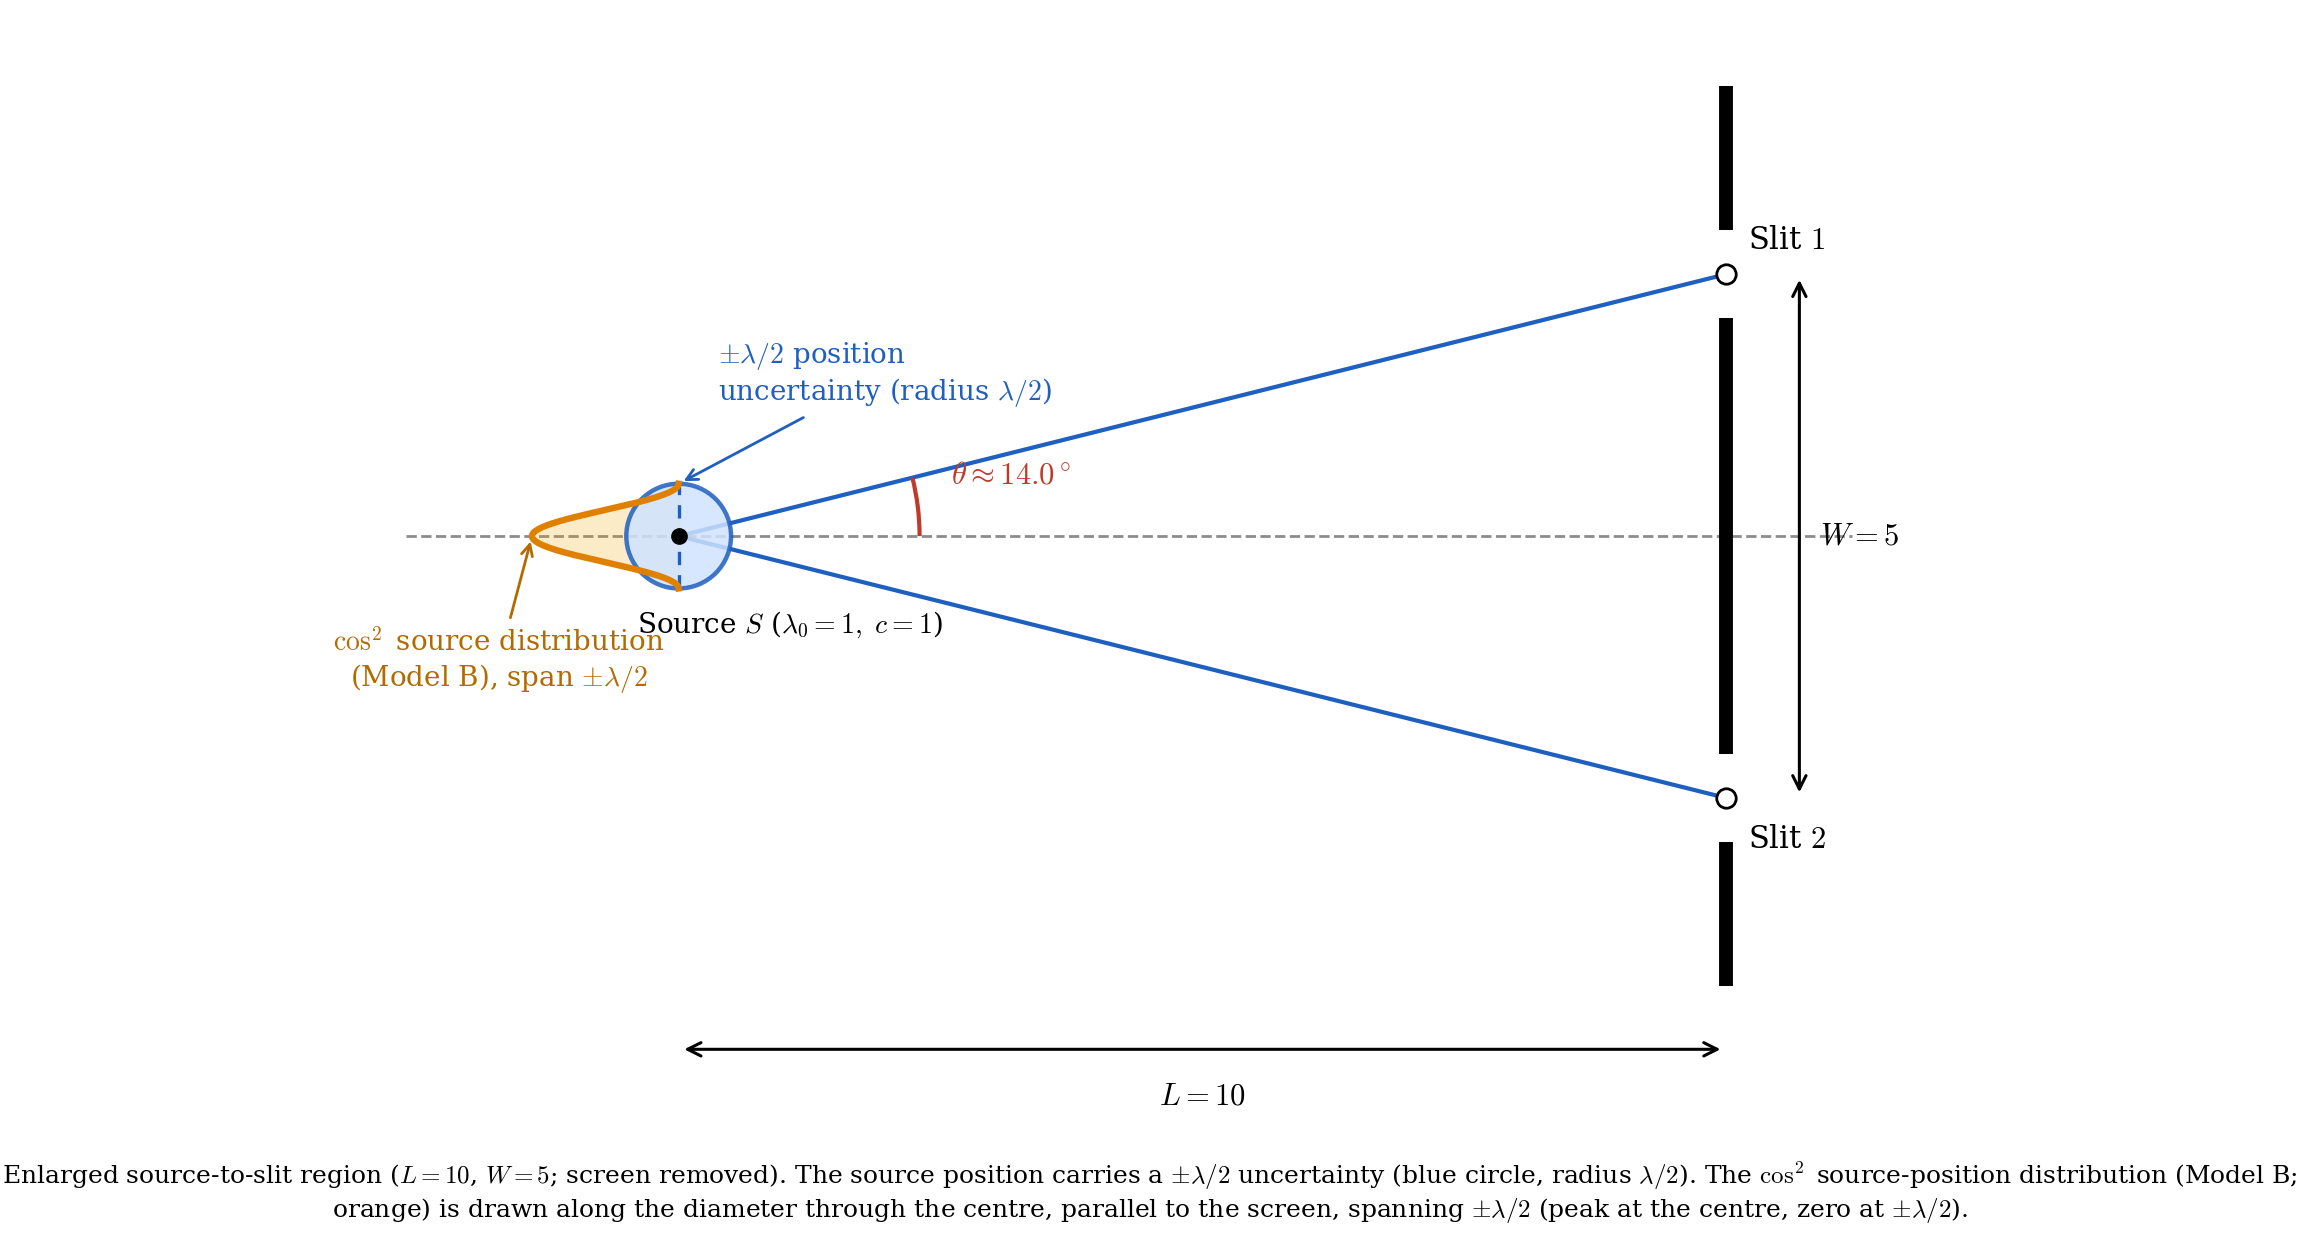
\includegraphics[keepaspectratio,alt={Fig 2 positional fluctuation of the source}]{fig_setup_source_uncertainty.png}}
\caption{Fig 2 positional fluctuation of the source}
\end{figure}

\emph{Fig 2: Magnified view of the source--slit region (\(L=10\),
\(W=5\); the screen is removed). The source position has an uncertainty
disc of radius \(\lambda/2\) (blue); along the axis through its center,
parallel to the screen, rides the distribution \(P(y)=\cos^2\) (orange;
\(\pm\lambda/2\), central peak, zero at the ends).}

\begin{center}\rule{0.5\linewidth}{0.5pt}\end{center}

\subsection{3. Method (pure geometric
model)}\label{method-pure-geometric-model}

Let the source be \(S=(-L,\,y)\) and the slits \(A_1=(0,+W/2)\),
\(A_2=(0,-W/2)\). The screen point is parametrized by the far-field
diffraction angle \(\theta_s\) (\(s=\sin\theta_s\)). The wavelength is
\(\lambda_0\) everywhere (no motion assumption, no Doppler: the light
propagates at \(c\) from a stationary source, and since the emission
point does not move, no frequency shift occurs).

The phase of each arm \(k\) is the sum of the source-side geometric path
and the far-field screen-side path difference:

\[\Phi_k(s;y)=\frac{2\pi}{\lambda_0}\Big[\,r_k(y)-y_{{\rm slit},k}\,s\,\Big],\qquad
r_k(y)=\sqrt{L^2+(y-y_{{\rm slit},k})^2}.\]

The interference intensity (exact Born form via complex conjugation) is

\[I(s;y)=\big|e^{i\Phi_1}+e^{i\Phi_2}\big|^2
=2+2\cos\!\Big[\tfrac{2\pi}{\lambda_0}\big(\Delta r(y)-W s\big)\Big],\qquad \Delta r(y)=r_1-r_2.\]

Only the phase offset \(\Delta r(y)\) depends on \(y\); the
\textbf{waveform is exactly identical in shape} (``identical shape,
merely shifted'' is exact, not an approximation). The position of the
central peak (\(\Delta\Phi=0\)) is

\[u(y)\equiv\Phi_0^{\rm peak}(y)=\frac{2\pi}{\lambda_0}\,\Delta r(y)\ \approx\ -\frac{2\pi W}{L\lambda_0}\,y\quad(\text{linear in the paraxial regime})\]

(the horizontal axis is the slit-reference phase
\(\Phi_0=2\pi W s/\lambda_0\)).

\begin{center}\rule{0.5\linewidth}{0.5pt}\end{center}

\subsection{4. Results}\label{results}

\subsubsection{4.1 Shift distribution =
push-forward}\label{shift-distribution-push-forward}

Drawing the interference for each source position separately, each trial
shifts a fringe of identical shape by \(u(y)\) (Fig 3). The probability
distribution of the shift \(u\) is the push-forward of \(P\),

\[\rho(u)=P\big(y(u)\big)\,\Big|\frac{dy}{du}\Big|.\]

If \(u(y)\) is linear then \(|dy/du|\) is constant, and
\textbf{\(\rho(u)\) has the same shape as \(P\) (only the axis is
rescaled). This is not a property special to \(\cos^2\) but a
consequence of a linear map preserving the shape of any input \(P\).}
For our example \(P=\cos^2(\pi y/\lambda)\),
\(\rho(u)\propto\cos^2(\pi u/180^\circ)\).

\begin{figure}
\centering
\pandocbounded{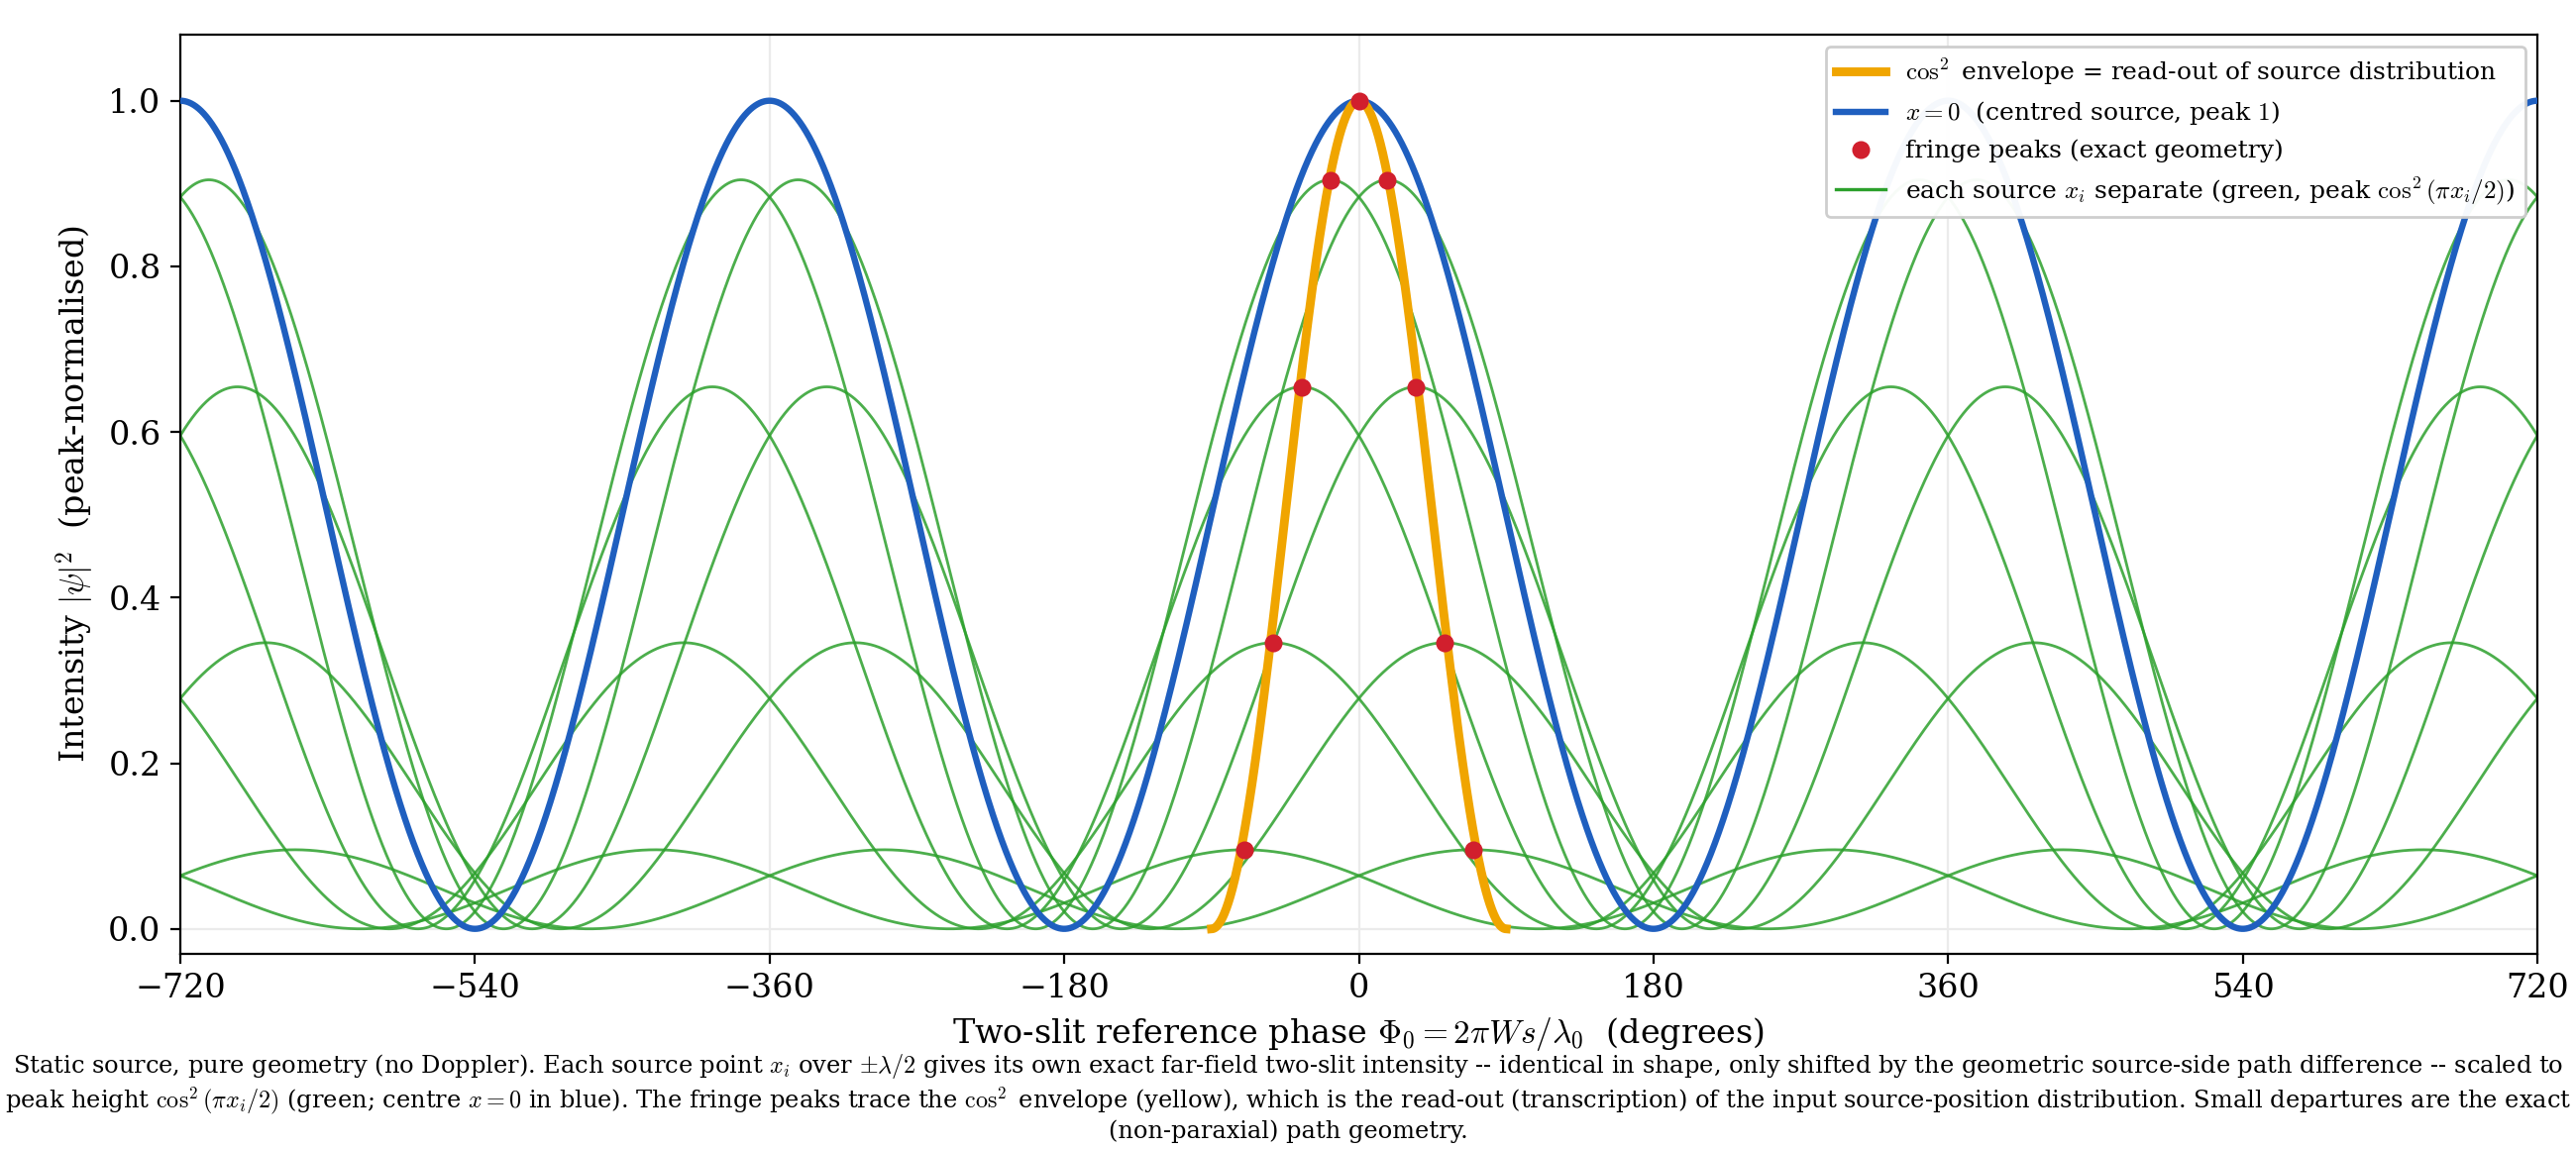
\includegraphics[keepaspectratio,alt={Fig 3 fringes for each source position (identical-shape shift)}]{fig_decomposition_static.png}}
\caption{Fig 3 fringes for each source position (identical-shape shift)}
\end{figure}

\emph{Fig 3: Stationary source, pure geometry (no Doppler). The exact
far-field two-slit intensity for each source position \(x\) is
\textbf{identical in shape, merely shifted by the source-side path
difference}. The peak height of each waveform is the weight
\(\cos^2(\pi x/2)\) (green; the central \(x=0\) in blue). The fringe
peaks (red dots) of the waveforms trace the \(\cos^2\) envelope
(yellow).}

We confirm this directly by a Monte-Carlo of repeated trials. Drawing
\(y\) from \(P(y)\) and \textbf{reading only the fringe shift \(u(y)\)}
each trial and histogramming (Fig 4), \(\rho(u)\) preserves the
\(\cos^2\) shape.

\begin{figure}
\centering
\pandocbounded{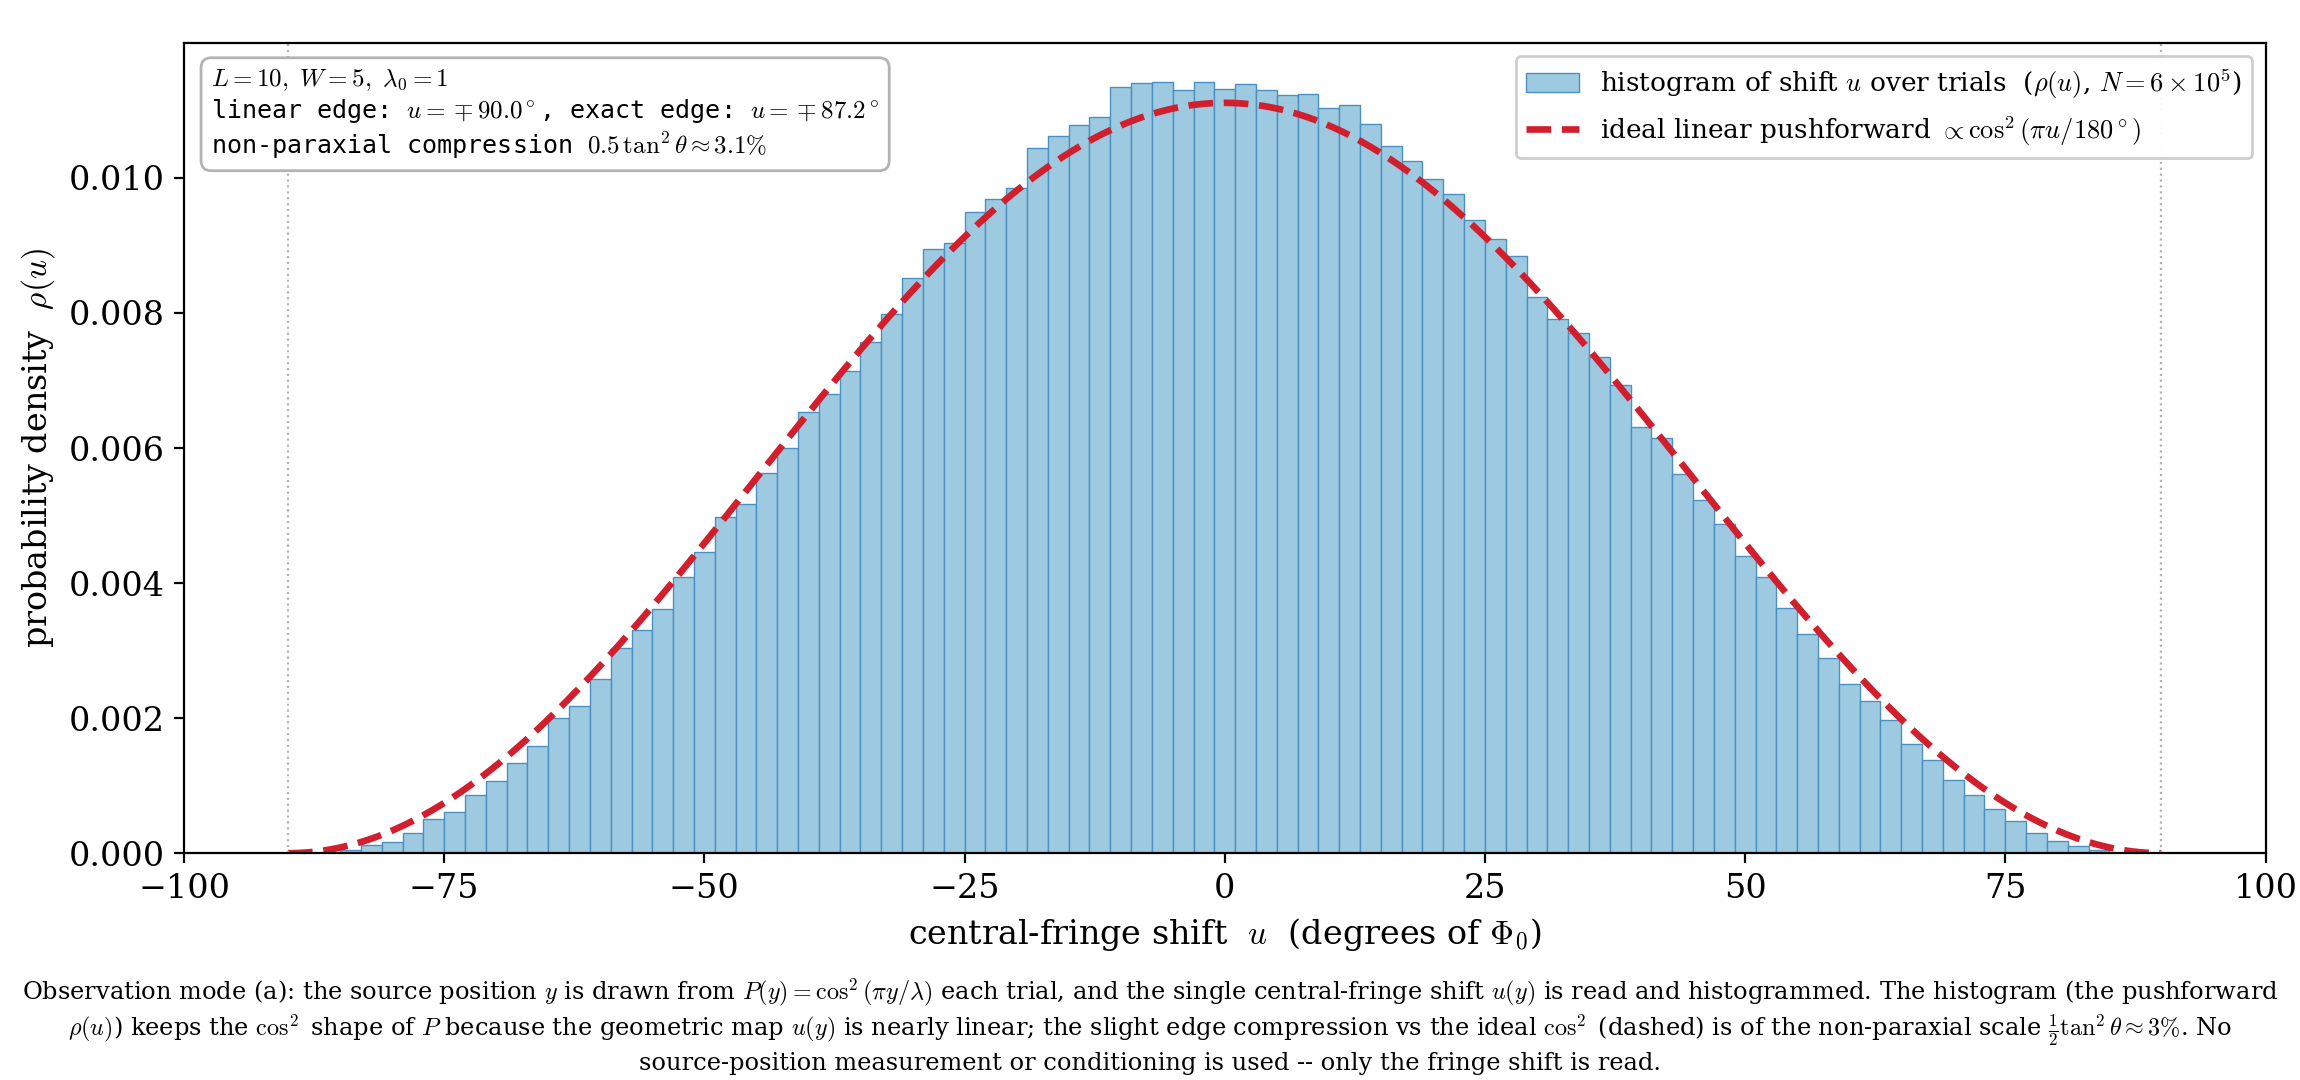
\includegraphics[keepaspectratio,alt={Fig 4 histogram of the shift (push-forward)}]{fig_shift_histogram.png}}
\caption{Fig 4 histogram of the shift (push-forward)}
\end{figure}

\emph{Fig 4: Observation mode (a). Each trial draws \(y\sim P(y)\) and
reads the single fringe shift \(u(y)\), histogrammed
(\(N=6\times10^5\)). The histogram \(\rho(u)\) preserves the \(\cos^2\)
shape of \(P\) (because the map \(u(y)\) is nearly linear). The edge
compression relative to the ideal \(\cos^2\) (red dashed) (exact edge
\(u=\mp87.2^\circ\) vs linear \(\mp90^\circ\), \(3.09\%\)) is the
non-paraxial nonlinearity (scale \(\tfrac12\tan^2\theta\approx3\%\)). No
source-position measurement or conditioning is used; only the fringe
shift is read.}

\subsubsection{4.2 Uniqueness (aliasing
condition)}\label{uniqueness-aliasing-condition}

The shift \(u\) is the position of the central (zeroth-order) fringe,
and in this configuration stays within
\(|u|\le u_{\max}=\dfrac{\pi W}{L}=90^\circ<180^\circ\) (half of the
fringe period \(360^\circ\)). Hence the zeroth-order fringe does not mix
with the adjacent orders (\(\pm360^\circ\)), and the shift can be read
uniquely. If \(W/L\) or the source swing is large enough that
\(u_{\max}\ge180^\circ\), the map wraps around (aliases) and the
histogram folds back. The push-forward of this paper holds within this
uniqueness range.

\subsubsection{4.3 Quantifying the
departure}\label{quantifying-the-departure}

The departure from \(\cos^2\) (at most \(\sim3\%\) at the edges) arises
from the non-paraxial nonlinearity of the map \(u(y)\). Expanding the
source-side path difference, the slope correction at the center is
\(\tfrac12\tan^2\theta=\tfrac12(0.25)^2=3.13\%\). The Monte-Carlo edge
compression is \(3.09\%\); because it includes quartic and higher terms
at the edge it is not exactly the same quantity as
\(\tfrac12\tan^2\theta\), but it is of the same non-paraxial scale
(\(\approx3\%\)) and consistent. In the paraxial limit \(W/L\to0\),
\(u(y)\) becomes exactly linear and the shape preservation becomes
exact.

\begin{center}\rule{0.5\linewidth}{0.5pt}\end{center}

\subsection{5. Discussion}\label{discussion}

\subsubsection{5.1 Stating the observation mode --- what is the
push-forward of
what}\label{stating-the-observation-mode-what-is-the-push-forward-of-what}

The distribution in this paper is \textbf{not a property of a single
observed image}. Two observation modes must be distinguished.

\begin{itemize}
\tightlist
\item
  \textbf{(a) Read the fringe shift (central-peak position) each trial
  and build a histogram over repetitions} \(\rightarrow\) the
  push-forward of \(P\) (Fig 4). This is the claim of this paper. The
  source position \(y\) need not be measured directly; since the fringe
  position encodes \(y\), it suffices to read the shift.
\item
  \textbf{(b) Accumulate the intensity of many trials on one screen}
  \(\rightarrow\) a \textbf{single fringe of reduced visibility}
  convolved with the shift (\(2+2V\cos\), \(V<1\)), which is not the
  shape of the input distribution.
\end{itemize}

A single trial yields one shift (one fringe), not a distribution. The
shape appears as the statistic of repeated trials (an ensemble). This
requires the source position to be \textbf{quasi-static within a trial
(fixed while the fringe forms) and to fluctuate between trials} (if the
fluctuation is fast within a trial, mode (b) results and the shape
vanishes). What one obtains is not a ``derived distribution'' but the
\textbf{push-forward (change of variables)} by which the input \(P(y)\)
is mapped to the shift distribution.

\subsubsection{5.2 On inertial frames (limited
remark)}\label{on-inertial-frames-limited-remark}

If the same experiment is constructed in any inertial frame (at rest in
that frame), the relativity principle gives the same shift statistics.
This is a trivial consequence of the relativity principle, and we claim
nothing beyond it. In particular, we do \textbf{not} assert the strong
statement that ``because the set of detection events is
Lorentz-invariant, the transcription relation holds even when one
experiment is viewed by a moving observer'' (the quantitative fringe
spacing is frame-dependent via aberration etc., and consistency of the
transformations on both sides requires a separate calculation).

\subsubsection{5.3 Translation of the source itself is a separate
problem (out of
scope)}\label{translation-of-the-source-itself-is-a-separate-problem-out-of-scope}

This paper treats a stationary source whose emission point does not
move. A setting in which the source itself translates (transverse
velocity \(\beta_{\rm src}<1\)) is a separate problem in which the two
slits receive different Doppler frequencies and the visibility loss due
to that frequency mismatch competes with the shift readout; it is out of
scope (future work).

\subsubsection{5.4 Relation to the classical picture (arcsine) ---
making the coordinate
explicit}\label{relation-to-the-classical-picture-arcsine-making-the-coordinate-explicit}

If the source is regarded as a classical point \(e^{i\theta}\) moving
uniformly on a circle of radius \(\lambda/2\), the resulting
distribution \textbf{depends on which coordinate one views it in}.

\begin{itemize}
\tightlist
\item
  \textbf{Projected coordinate \(x=\sin\theta\)}: the projection of
  uniform \(\theta\) is the arcsine law \(p_A(x)=1/(\pi\sqrt{1-x^2})\)
  (a U-shape diverging at the ends). Multiplying by the
  amplitude-squared weight (Born factor \(\cos^2\theta=1-x^2\)) gives
  \(p\propto\sqrt{1-x^2}\) = a \textbf{semicircle}, not \(\cos^2\).
\item
  \textbf{Arc-length coordinate \(\theta\) (the \(y\) of this paper,
  \(\theta=\pi y/\lambda\))}: uniform \(\to\) uniform. Multiplying by
  the Born factor \(\cos^2\theta\) gives \(\cos^2\theta\). The \(P(y)\)
  of this paper is the latter.
\end{itemize}

That is, the arcsine lives in the projected coordinate \(x\) and
\(\cos^2\) in the arc-length coordinate \(\theta\); they are \textbf{not
related by the Born factor in the same coordinate} (a change of
coordinate is involved). Robinett (1995) {[}1{]} shows that the
classical probability density of the harmonic oscillator is arcsine-type
and that the quantum \(|\psi_n|^2\) approaches it in the large-\(n\)
limit; this is the standard backing for the arcsine (projected
coordinate, high-\(n\) correspondence of the classical HO) and is not
directly identified with the \(\cos^2\) (arc-length coordinate) of this
paper.

\begin{center}\rule{0.5\linewidth}{0.5pt}\end{center}

\subsection{6. Conclusion}\label{conclusion}

For double-slit interference from a stationary source with positional
fluctuation, exact pure-geometry computation shows the following.

\begin{enumerate}
\def\labelenumi{\arabic{enumi}.}
\tightlist
\item
  In a single trial, the fringe shifts left or right by \(u(y)\) while
  remaining \textbf{exactly identical in shape} (constant wavelength, no
  waveform deformation).
\item
  When the source position \(y\) is repeatedly drawn from a distribution
  \(P(y)\), \textbf{the probability distribution of the fringe shift
  \(u\) is the push-forward of \(P\), and because the map \(u(y)\) is
  linear in the paraxial regime, the shape of \(P\) is preserved}. This
  is not special to \(\cos^2\) but a general consequence of a linear
  map; we showed with \(P=\cos^2\) that the same-shape \(\cos^2\)
  results. The departure from the shape (\(\sim3\%\)) arises from the
  non-paraxial nonlinearity of the map (scale
  \(\tfrac12\tan^2\theta\approx3\%\)) and vanishes in the paraxial
  limit. The shift is unique within \(|u|<180^\circ\) (no aliasing).
\item
  This distribution is a \textbf{statistic of repeated-trial shifts},
  not a single observed image, nor an intensity-accumulated single image
  (whose visibility is reduced and whose shape is lost).
\end{enumerate}

This is not the derivation of a new probability law but an illustration
that the input distribution is mapped onto the observed statistic
(fringe shift), \textbf{preserving its shape}, by the paraxial linear
geometric map. This paper is a thought experiment; it illustrates and
organizes established physics rather than overturning it.

\begin{center}\rule{0.5\linewidth}{0.5pt}\end{center}

\subsection{References}\label{references}

{[}1{]} R. W. Robinett, ``Quantum and classical probability
distributions for position and momentum,'' \emph{American Journal of
Physics} \textbf{63}(9), 823--832 (1995). DOI: 10.1119/1.17807.

{[}2{]} M. Born and E. Wolf, \emph{Principles of Optics}, 7th (expanded)
ed.~(Cambridge University Press, 1999).

\begin{center}\rule{0.5\linewidth}{0.5pt}\end{center}

\emph{(Reproduction code: \texttt{fig\_setup\_double\_slit.py},
\texttt{fig\_setup\_source\_uncertainty.py},
\texttt{fig\_decomposition\_static.py},
\texttt{fig\_shift\_histogram.py}. All angles and paths are derived from
\(L,W\); no constants are placed arbitrarily. No motion assumption or
Doppler is used.)}

\end{document}
